\section{System Description}

\subsection{Notation}
A set $\mathcal{S}$ of points $\mathbf{x}\in\mathbb{R}^{2}$ is defined by it's boundary, $\delta\mathcal{S}$, 
and it's interior, $\mathrm{int}(\mathcal{S})$. The number of elements in a set $\mathcal{S}$ is denoted as $|\mathcal{S}|$.\newline
The $Comb(\cdot)$ operator takes as arguments a set $\mathcal{S}$ and an integer $n$ and returns all subset of $\mathcal{S}$ of lenght $n$:
\begin{equation}
  Comb(\mathcal{S}, n) = \{\mathcal{A}: \mathcal{A}\subseteq\mathcal{S}, |\mathcal{A}|=n\}
\end{equation}

\subsection{Feasible space}
As in \cite{sun2014escaping}, a \textit{mission space}, $\Omega$, is defined as a simple polygon 
\cite{weissteinsimplepolygon}.
Within the mission space there exists $N_{o}\geq 0$ obstacles, each one of which is defined as a simple polygon.
The set of all obstacles, $\mathcal{O}$, is defined according to \eqref{obstacle_set_def}.
\begin{equation}\label[eq]{obstacle_set_def}
  \mathcal{O} = \begin{cases}
    \{o_{0}\hdots o_{N_{o}-1}\} &, N_{o} > 0\\
    \emptyset &, N_{o} = 0\\
  \end{cases}
\end{equation}
The obstacles in $\mathcal{O}$ constrains the movement of entities within the mission space, as it is not possible to
penetrate the boundary of an obstacle. Due to this, once an entity is inside $\Omega$, it is constrained to be positioned within
$\Omega$ and outside $\mathrm{int}(o)\;\forall\;o\in\mathcal{O}$. From this we define the \textit{feasible space}, $\mathcal{F}$, as
all points where it is possible to place an entity:
\begin{equation}\label[eq]{feasible_space_def}
  \mathcal{F} = \{\mathbf{x}\in\mathbb{R}^{2}: \mathbf{x}\in\Omega,\;\mathbf{x}\notin\mathrm{int}(o)\;\forall\;o\in\mathcal{O}\} = \Omega\setminus\bigcup_{o\in\mathcal{O}}\mathrm{int}(o)
\end{equation}

\subsection{Agent}
An \textit{agent}, denoted by an integer $i$, is described by its position $\mathbf{s}_{i}\in\mathbb{R}^{2}$ and 
it's maximum radius of communication, $r_{i}$.
The probability of an agent $i$ being able to communicate with another entity positioned at a point $\mathbf{x}$ is defined according to:
\todo{Find notation for $\mathbb{R}^{5}$ with non-negative values in last dimension}
\begin{equation}
  \hat{p}:(\mathbb{R}^{2}, \mathbb{R}^{2}, \mathbb{R}^{+})\rightarrow [0, 1]\quad\hat{p}(\mathbf{s}_{i}, \mathbf{x}, r_{i}) = \begin{cases}
    p(\norm{\mathbf{s}_{i}-\mathbf{x}}) &, \mathbf{x}\in V(\mathbf{s}_{i}, r_{i})\\
    0 &, \mathbf{x}\in\mathbb{R}^{2}\setminus V(\mathbf{s}_{i}, r_{i})
  \end{cases}
\end{equation}
Where $V(\mathbf{s}_{i}, r_{i})$ denotes the \textit{visible set} of agent $i$. Assuming line-of-sight (LoS) communication, meaning an agent
cannot communicate with an entity if there is an obstacle or a mission space wall between them, the visible set of agent 
$i$ is defined in \eqref{visible_set_def}.
\begin{equation}\label[eq]{visible_set_def}
  V(\mathbf{s}_{i}, r_{i}) = \{\mathbf{x}\in\mathbb{R}^{2}:\norm{\mathbf{s}_{i}-\mathbf{x}}\leq r_{i}, \lambda\mathbf{x} + (1-\lambda)\mathbf{s}_{i}\in\mathcal{F}\;\forall\;0\leq\lambda\leq 1\}
\end{equation}
An example of the visible set for an agent is show in \figref{vis_set_example}.
\begin{figure}[H]
  \centering
  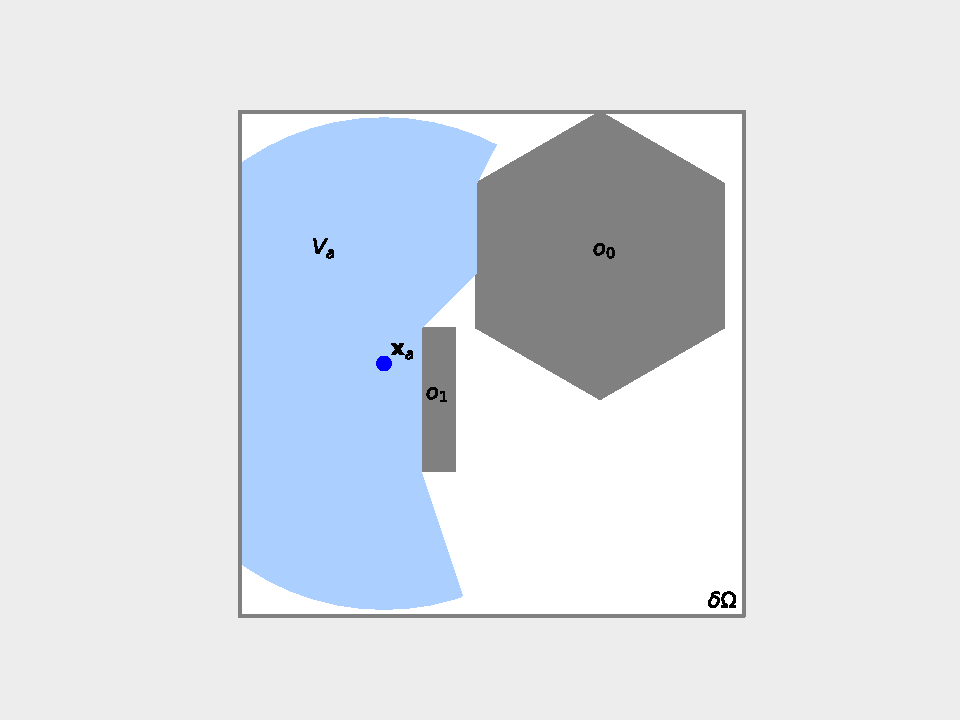
\includegraphics[width=\textwidth]{figs/vis_set_example.pdf}
  \caption{Visible set (light blue) for the agent placed at $\mathbf{s}_{i}$ in a rectangular mission space $\Omega$ with two obstacles ($\mathcal{O} = \{o_{0}, o_{1}\}$)}
  \label[fig]{vis_set_example}
\end{figure}
\subsection{Swarm}
A \textit{swarm} consists if $N$ discinct agents, each one denoted by an integer $i\in\mathcal{N}=\{0\hdots N-1\}$. The state of the swarm is described by the state of its participants 
, and is expressed as vector $\mathbf{S}\in\mathbb{R}^{2N}$ as shown in \eqref{swarm_state_def}.
\begin{equation}\label[eq]{swarm_state_def}
  \mathbf{S} = \begin{bmatrix}
    \mathbf{s}_{0}\\\vdots\\\mathbf{s}_{N-1}
  \end{bmatrix}
\end{equation}
The maximum radii of communication of the swarm are represented as the vector $\mathbf{r}\in\mathbb{R}^{N}$ as shown in \eqref{swarm_radii_def}.
\begin{equation}\label[eq]{swarm_radii_def}
  \mathbf{r} = \begin{bmatrix}
    r_{0}&\hdots&r_{N-1}
  \end{bmatrix}^{T}
\end{equation}
Assuming that the distributions for all agents are independent lets us use (7) in \cite{10.2307/24304959} to express 
the probability of $n$ members in the swarm being able to communicate with an entity at a point $\mathbf{x}$:
\begin{equation}
  P(n, \mathbf{x}, \mathbf{S}, \mathbf{r}) = \sum_{A\in Comb(\mathcal{N}, n)}\Bigg(\prod_{i\in\mathcal{A}}\hat{p}(\mathbf{s}_{i}, \mathbf{x}, r_{i})\Bigg)\Bigg(\prod_{i\in\mathcal{N}\setminus\mathcal{A}}1-\hat{p}(\mathbf{s}_{i}, \mathbf{x}, r_{i})\Bigg)
\end{equation}